\documentclass[a4paper,usenatbib]{aspdoc}
\usepackage{newtxtext,newtxmath}
\usepackage{ae,aecompl}
\usepackage{graphicx}	% Including figure files
\usepackage{amsmath}	% Advanced maths commands
\usepackage{amssymb}	% Extra maths symbols
\usepackage{lipsum}
\usepackage{float}
\usepackage{multirow}
\usepackage{booktabs}
\usepackage{geometry}
\usepackage{bm}
\usepackage[load=prefixed]{siunitx}
\sisetup{output-decimal-marker = {,}}
\geometry{left=25mm,right=25mm,top=25mm,bottom=25mm}

\newcounter{simplecount}
\setcounter{simplecount}{0}
\renewcommand{\theequation}{\arabic{simplecount}}
\newcommand{\owncount}{\refstepcounter{simplecount}}

\usepackage{subcaption}
\usepackage{subfig}
%\usepackage{subfigure}
%\usepackage[T1]{fontenc}
%\usepackage{blindtext}

% Title
\title[]{OSZ: Aufnahme von Durchlasskurven mit dem Oszilloskop}

% The list of authors
\author[]{
    Riedel Lisa, Wegmann Peter
    \newauthor
    \,Gruppe 6
}
% Don't change these lines
\begin{document}
    \label{firstpage}
    \pagerange{\pageref{firstpage}--\pageref{lastpage}}
    \maketitle
    
    

    % Body
    \section{Einleitung}\label{sec:intro}
        Das Oszilloskop ist ein wichtiges Instrument zur Messung von Wechselspannungen. Bei diesem Versuch beschäftigte man sich mit dem Messen von Durchlasskurven und Phasenverschiebungen, sowie der Bestimmung von Eigenschaften verschiedener Schwingkreise.

        \subsection{Tastkopf}
            Die Spannungsmessung mit dem Oszilloskop kann aufgrund des Eigenwiderstandes und der Eigenkapazität verfälscht werden. Um dem Entgegenzuwirken wird ein Tastkopf verwendet, da dieser das Messsignal abfangen kann, und dabei die ohmsche und kapazitive Belastung möglichst gering hält. 
            
            \subsubsection{Funktionsweise}
                Die Funktionsweise eines Tastkopf wird mit Hilfe von Abbildung \ref{fig:tast} erklärt. Auf der Abbildung sind zwei Spannungsteiler zu erkennen. Die beiden Widerstände bilden einen ohmschen, die beiden Kapazitäten einen komplexen Spannungsteiler. Diese beiden Teiler sind über eine Brücke miteinander verbunden, über die, bei unterschiedlichen Teilverhältnissen, Ausgleichsströme fließen. Bei gleichen Verhältnissen fließt kein Strom. \\
                Das bedeutet, wenn das Verhältnis zwischen komplexen und ohmschen Spannungsteiler gleich ist, fließt kein Strom über die Brückenverbindung, die Spannungsteiler beeinflussen sich nicht gegenseitig und das Messsignal wird nicht verfälscht.\\
                \begin{figure}
                    \centering
                        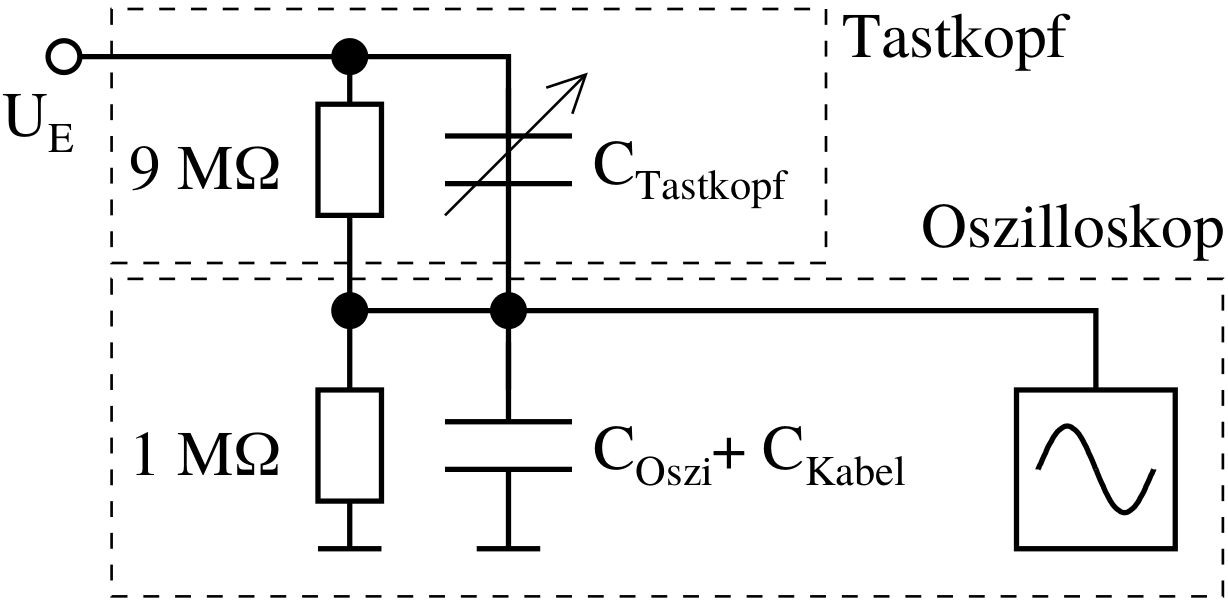
\includegraphics[width=0.47\textwidth]{pictures/tastkopf.png}
                        \caption{Schaltung eines Oszilloskop mit Tastkopf. Abbildung entnommen aus \citep{anleitung}.}
                    \label{fig:tast}
                \end{figure}
            
            \subsubsection{Berechnung der Kapazität des Tastkopfes}
                Damit der Tastkopf wie gewünscht funktioniert, müssen die Verhältnisse der Spannungsteiler gleich sein. Die Kapazität des Kondensators ist variabel und kann mit Hilfe des Oszilloskop eingestellt werden. Die Kapazität lässt sich mit der Verhältnisgleichung aus der Brückenschaltung berechnen. 
                
                \begin{equation}
                    \owncount
                    \frac{R_{Tastkopf}}{R_{Oszi}} = \frac{C_{Tastkopf}}{C_{Oszi+Kabel}} \\
                \end{equation}
                \\
                Da es sich bei $C_{Tastkopf}$ und $C_{Oszi+Kabel}$ um Kapazitäten handelt, muss der Kehrwert von $\frac{R_{Tastkopf}}{R_{Oszi}}$ genommen werden. Daraus ergibt sich dann die Kapazität des Tastkopfes für Abbildung \ref{fig:tast}.
                
                \begin{equation}
                    \owncount
                    \begin{aligned}
                        C_{Tastkopf} = \frac{R_{Oszi}}{R_{Tastkopf}}\cdot C_{Oszi+Kabel}  \\
                        \Leftrightarrow \mathbf{C_{Tastkopf} =  \frac{1}{9} \cdot C_{Oszi+Kabel}}
                    \end{aligned}
                \end{equation}
            
            
    \section{Verwendete Methoden}\label{sec:method}
        \subsection{Tiefpass}
            Die Berechnung der Grenzfrequenz $f_g$ kann durch Fitting folgender Theorifunktionen bestimmt werden.
            \begin{equation}
                \owncount
                g_{\mathrm{TP}} = \frac{1}{\sqrt{1+(\omega RC)^2}}
                \label{eq:durchlasskurve}
            \end{equation}
            \begin{equation}
                \owncount
                \varphi_{\mathrm{TP}} = \arctan(-\omega RC)
                \label{eq:phasenkurve}
            \end{equation}
            Dabei ist $R$ ein Widerstand, $C$ eine Kapazität, sowie $\omega$ die Kreisfrequenz.
            Hierbei wird in Kapitel \ref{subsec:result_tiefpass} jeweils $RC$ als Fitting-Parameter verwendet. Die Grenzfrequenz lässt sich anschließend durch Formel \ref{eq:grenz} berechnen.
            \begin{equation}
                \owncount
                f_{G} = \frac{1}{2\pi RC}
                \label{eq:grenz}
            \end{equation}
            
        \subsection{Serienschwingkreis}
            Im folgenden betrachte man die zwei Theoriefunktionen der Durchlasskurve und der Phasenverschiebungskurve des Serienschwingkreis.
            \begin{equation}
                \owncount
                g_{\mathrm{Schw}} = \frac{R_m}{\sqrt{R^2 + (\omega L - \frac{1}{\omega C})^2}}
                \label{eq:durchlasskurveSerie}
            \end{equation}
            \begin{equation}
                \owncount
                \phi = \arctan\left( \frac{1}{R} \left( \omega L - \frac{1}{\omega C} \right) \right)
                \label{eq:phasenkurveSerie}
            \end{equation}
            $L$ beschreibt dabei eine Induktivität. Unter Bezugnahme auf die durch die Theoriefunktionen berechneten Parameter, können weitere Eigenschaften der Schaltung berechnet werden.
            Die Berechnung der Resonanzfrequenz $f_{\mathrm{res}}$ wird mittels Formel \ref{eq:resonanzSerie} durchgeführt. Für den Serienschwingkreis liegt $f_{\mathrm{res}}$ bei der Eigenfrequenz $f_0$ des Systems, da die Dämpfung nicht sehr groß ist. 
            \begin{equation}
                \owncount
                f_0 = \frac{1}{2 \pi} \frac{1}{\sqrt{LC}}
                \label{eq:resonanzSerie}
            \end{equation}
            Bei der Bandbreite $B_{\mathrm{f}}$ handelt es sich um eine charakteristische Größe der Durchlasskurve und beschreibt die Differenz der Frequenzen zweier Punkte, an denen die Durchlasskruve auf das $1/\sqrt{2}$-fache ihres Maximalwerts abgesunken ist \citep{tipler}.
            \begin{equation}
                \owncount
                B_{\mathrm{f}} = \frac{R}{2 \pi L}
                \label{eq:bandSerie}
            \end{equation}
            Zudem lässt sich durch Bestimmung der Bandbreite der Gütefaktor $Q$ wie folgt bestimmen.
            \begin{equation}
                \owncount
                Q = \frac{f_{\mathrm{res}}}{B_{\mathrm{f}}}
                \label{eq:güteSerie}
            \end{equation}
            Eine andere Charakteristik, die Dämpfung des Serienschwingkreis, lässt sich durch Bestimmung der Dämpfungskonstante $\delta$ finden.
            \begin{equation}
                \owncount
                \delta = \frac{R}{2L}
                \label{eq:dampingSerie}
            \end{equation}
            
            
                % Figure moved up from subsec:result_tiefpass
                \begin{figure*}
                    \centering
                    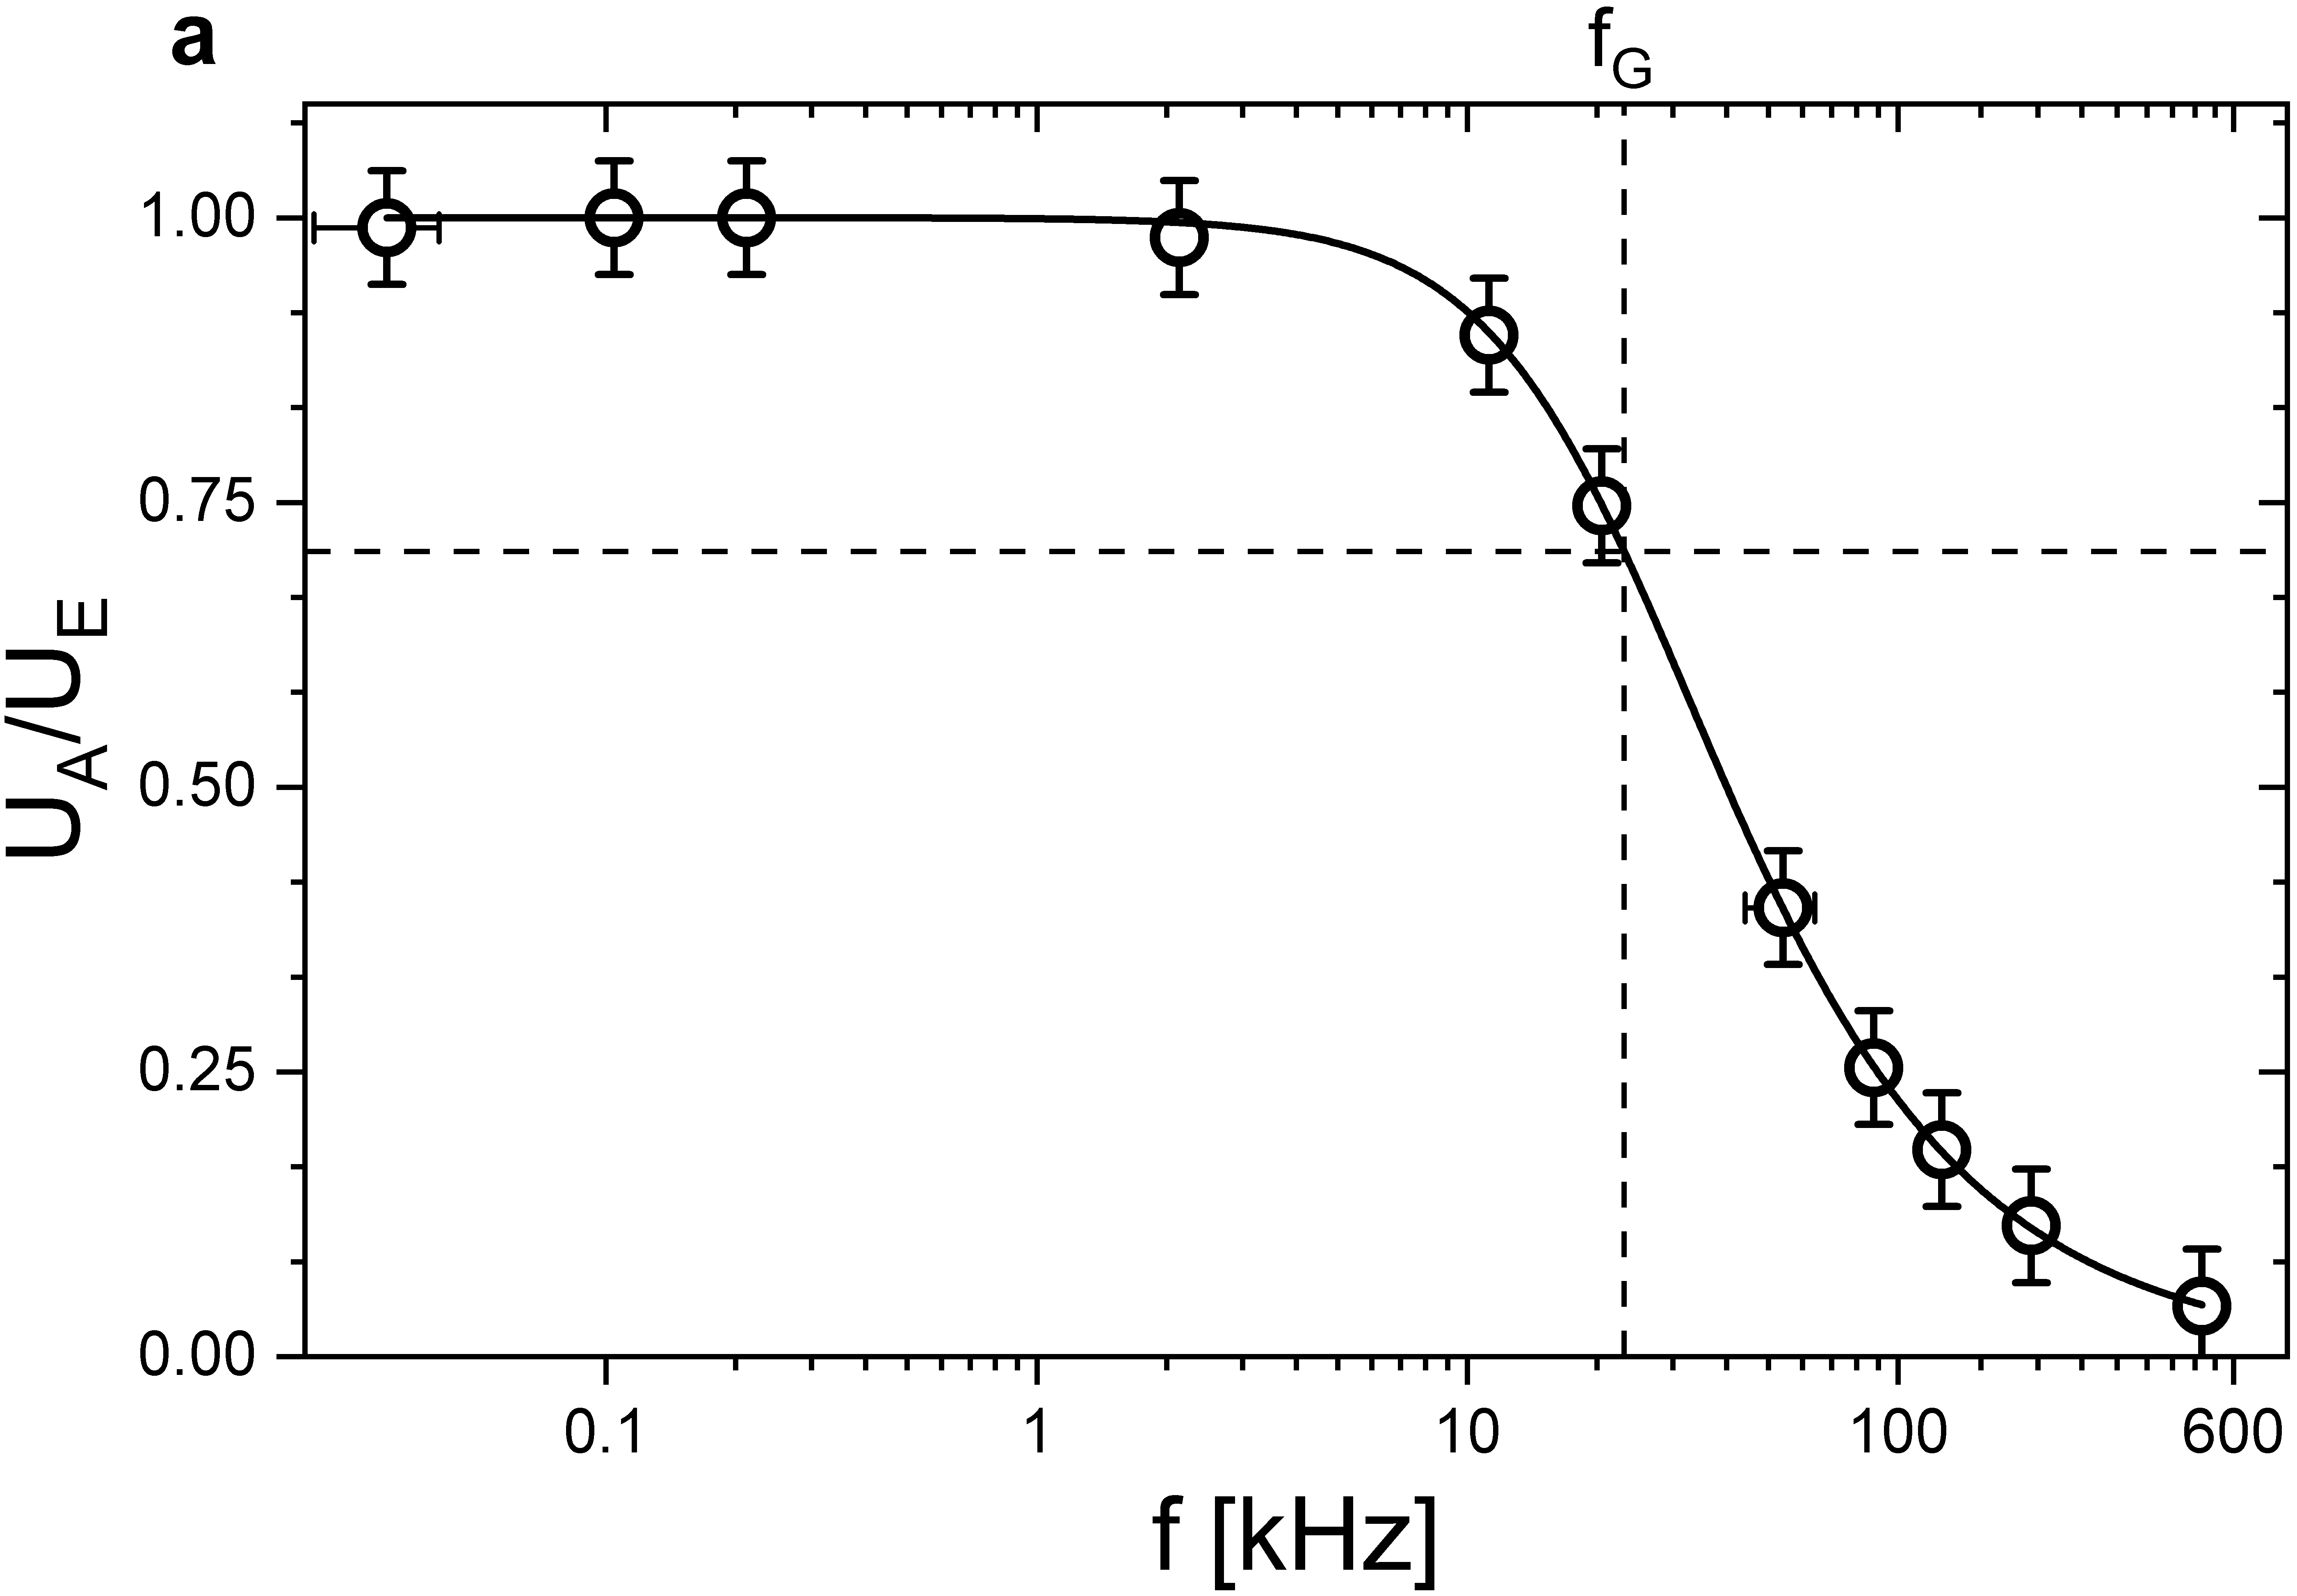
\includegraphics[width=79mm]{graphs/Durchlasskurv1.png}
                    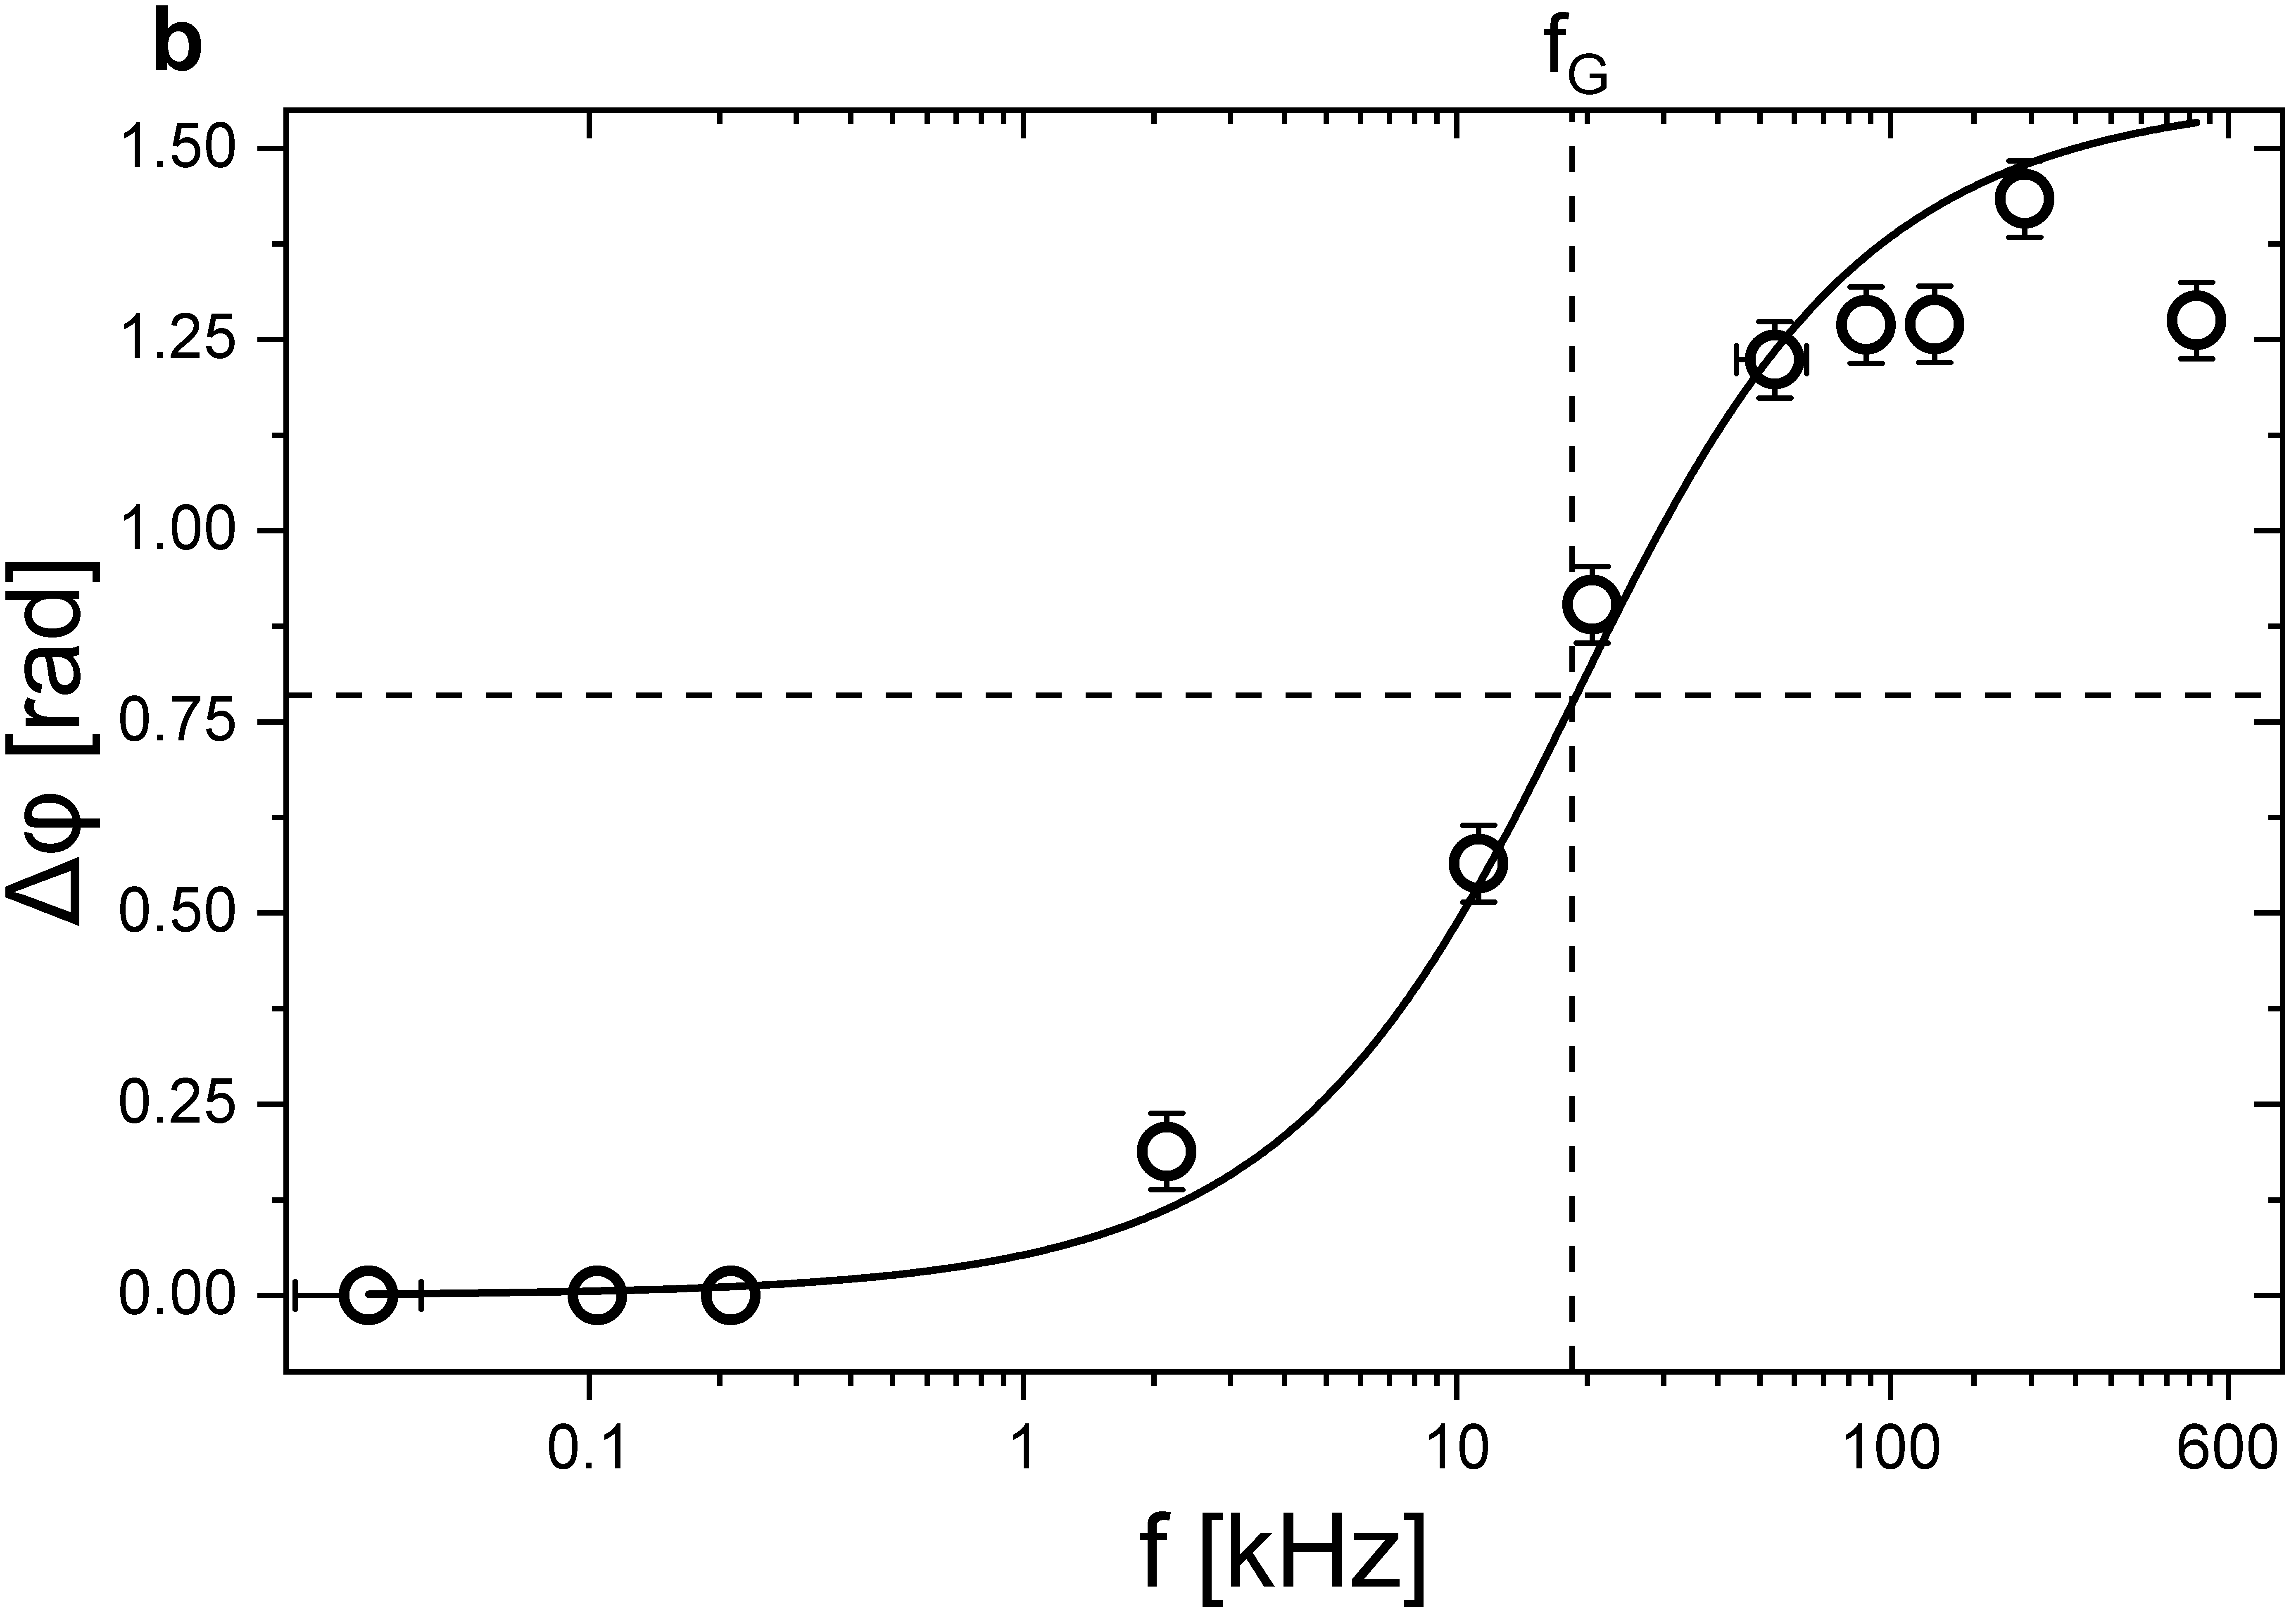
\includegraphics[width=79mm]{graphs/Phasenkurv1.png}
                    \caption{
                        \textbf{a} Durchlasskurve eines Tiefpass. Die berechnete Grenzfrequenz liegt hierbei bei $f_g \approx 23$ kHz.
                        \textbf{b} Phasenverschiebungskurve bezügliche Eingangs-/ und Ausgangssignal. Die berechnete Grenzfrequenz liegt hierbei bei $f_g \approx 18$ kHz. Man beachte hierbei, dass die Phasenverschiebung negativ ist, jedoch positiv dargestellt ist. \\
                        Bei beiden dargestellten Kurven handelt es sich um die Theoriefunktionen \ref{eq:durchlasskurve}-\ref{eq:phasenkurve}.
                    }
                    \label{fig:kurve}
                \end{figure*}
                
            
        \subsection{Koaxialkabel}
            Zur Berechnung der Resonanzfrequenz eines Parallelschwingkreises, mit vernachlässigbarer Dämpfung, kann folgende Formel verwendet werden. 
            \begin{equation}
                \owncount
                f_{res,S} = \frac{1}{2\pi}\sqrt{\frac{1}{L\cdot C_S}}
                \label{eq:grenzSerie}
            \end{equation}\\
            Hier ist $f_{res,S}$ die Resonansfrequenz, $L$ die Induktivität der verbauten Spule und $C_S$ die Kapazität des Schwingkreises. Möchte man nun die Kapazität berechnen, lässt sich die Gleichung in folgende Form umformen. 
            \begin{equation}
                \owncount
                C_S = \frac{1}{L\cdot(4\cdot\pi^2\cdot f_{res,S}^2)}
                \label{eq:kapschwing}
            \end{equation}\\
            Betrachtet man nun den Schwingkreis mit Koaxialkabel, lässt sich die Kapazität wie folgt beschreiben.
            \begin{equation}
                \owncount
                C_{KK} + C_S = \frac{1}{L\cdot(4\cdot\pi^2\cdot f_{res,KK}^2)}
                \label{eq:kapschwingkoax}
            \end{equation}\\
            Die Resonanzfrequenz von Parallelschwingkreis und Koaxialkabel ist hierbei $f_{res,KK}$. 
            
            
            
    \section{Experimentelles Vorgehen}\label{sec:experiment}
        Zu Beginn des Versuches wurde der Tastkopf kalibriert. Dafür wurde dieser an das Oszilloskop angesteckt und dessen Kapazität so lange verändert, bis das Signal keine Über- oder Oberspannung mehr anzeigte. \\
        Danach wurde die Durchlasskurve und die Phasenverschiebung eines Tiefpasses gemessen. Der Tiefpass wurde am Funktionsgenerator angeschlossen. Die Eingangs- und Ausgangsspannung wurde dann mit dem Oszilloskop visualisiert. Es wurde die Frequenz, die Eingangs- und Ausgangsspannung sowie die Zeitdifferenz der Amplituden notiert.\\
        Im nächsten Schritt wurde die differenzierende und integrierende Wirkung von Hoch- und Tiefpass untersucht. Hierfür wurde beim Hochpass eine sehr viel niedrigere Frequenz als die Grenzfrequenz am Funktionsgenerator eingestellt und das Eingangssignal als Dreieck- bzw. Rechtecksignal visualisiert. Beim Tiefpass wurde das selbe Verfahren angewendete, nur wurde eine sehr viel höhere Frequenz als die Grenzfrequenz eingestellt.\\
        Um die Durchlasskurve und die Phasenverschiebung des Serienschwingkreises zu messen, wurde zuerst die Resonanzfrequenz ermittelt. Danach wurde im Bereich von etwa $\pm 30\%$ der Resonanzfrequenz die Durchlasskurve und Phasenverschiebung gemessen. Hierfür wurde die Frequenz, die Eingangs- und Ausgangsspannung und die Zeitdifferenz der Amplituden notiert.\\
        Damit die reale Dämpfung des Serienschwingkreises ermittelt werden kann, wurde ein Rechtecksignal von etwa \SI{1}{\kilo\hertz} am Eingangssignal angelegt. Die angeregte, gedämpfte Schwingung wurde am Oszilloskop beobachtet und möglichst viele Amplituden mit deren Zeitabstand notiert. \\
        Zuletzt wurde mit Hilfe eines Parallelschwingkreises die Eigenkapazität eines \SI{10}{\metre} langen Koaxialkabels bestimmt. Dafür wurde über den Ausgang des Parallelschwingkreises der abgeglichene Tastkopf mit dem Oszilloskop verbunden. Durch durchfahren der Frequenzen mit dem Funktionsgenerator wurde die Resonanzfrequenz bestimmt. Als nächstes wurde zwischen Ausgang des Schwingkreises und dem Eingang des Tastkopfes das Koaxialkabel gesteckt. Durch erneutes durchfahren der Frequenzen konnte die Resonanzfrequenz des Kabels mit Schwingkreis bestimmt werden.

        
            
    \section{Ergebnisse}\label{sec:result}
        \subsection{Tiefpass}\label{subsec:result_tiefpass}
            Eine wichtige Charakteristik eines Tiefpass ist die Grenzfrequenz $f_g$. Hierbei handelt es sich um eine Art Barriere, wobei Frequenzen kleiner als $f_g$ den Tiefpass ungeschwächt passieren können. Frequenzen größer als $f_g$ werden durch den Tiefpass geschwächt. Dieser Vorgang der Schwächung von verschiedenen Frequenzen ist in Abbildung \ref{fig:kurve} dargestellt.
            \\
            Die Grenzfrequenz kann auf zwei verschiedenen Arten bestimmt werden. Bei der ersten wird $f_g$ durch Fitting der Theoriefunktion \ref{eq:durchlasskurve} in Abbildung \ref{fig:kurve}a bestimmt. Dabei wird $RC$ in der Theoriefunktion als freier Parameter betrachtet. Unter Verwendung von Funktion \ref{eq:grenz} ergibt dies 
            \begin{center}
                $\mathbf{f_g = (23,09 \pm 0,19)}$ \textbf{kHz} $\quad$.    
            \end{center}
            Die Grenzfrequenz lässt sich auch durch Fitting der Theoriefunktion \ref{eq:phasenkurve} in Abbildung \ref{fig:kurve}b bestimmen. Hierbei handelt es sich um die Phasenverschiebungskurve. Man wählt $RC$ als freien Parameter. Erneute Anwendung von Funktion \ref{eq:grenz} ergibt 
            \begin{center}
                $\mathbf{f_g = (18,44 \pm 2,53)}$ \textbf{kHz} $\quad$.    
            \end{center}
            \\
            Eine theoretische Berechnung von $f_g$ lässt sich unter Verwendung von Formel \ref{eq:grenz} und der Eigenschaften der verwendeten Bauteile berechnen. Der Tiefpass in diesem Versuch besitzt $R = 68$ $\Omega$ und $C = 100$ nF. Dies gibt eine theoretische Grenzfrequenz von 
            \begin{center}
                $\mathbf{f_g = (23,40 \pm 4,68)}$ \textbf{kHz} $\quad$.    
            \end{center}
            
        
        \subsection{Serienschwingkreis}\label{subsec:result_serie}
            Im folgenden berechnet man verschiedenen Charakteristiken eines Serienschwingkreis mittels experimentell bestimmter Ergebnisse, sowie durch Verwendung der Eigenschaften der verwendeten Bauteile.
            \\
            Die Berechnung der gesuchten Parameter wird mittels Fitting der Theoriefunktion \ref{eq:durchlasskurveSerie} für die Durchlasskurve und Theoriefunktion \ref{eq:phasenkurveSerie} für die Phasenverschiebungskurve gelöst. Anschließend können die Resonanzfrequenz, Bandbreite und Güte mittels Formeln \ref{eq:resonanzSerie}-\ref{eq:güteSerie} berechnet werden. Dabei verwendet man die durch die Theoriefunktionen gefundenen Parameter für $R, L, C$.
            \\
            Die theoretische Berechnung oben genannter Charakteristiken lässt sich unter Verwendung der angegebenen Eigenschaften der Bauteile umsetzten. Der verwendete Serienschwingkreis besitzt $L = 4,7$ mH, $C = 560$ pF und $R = 300$ $\Omega$. Jeweiliges einsetzen dieser in die oben angeführten Formeln, ergeben die in Tabelle \ref{tab:serie} dargestellten Ergebnisse für $f_{\mathrm{res}}, B_{\mathrm{f}}$ und $Q$.
            
            \begin{figure*}
                \centering
                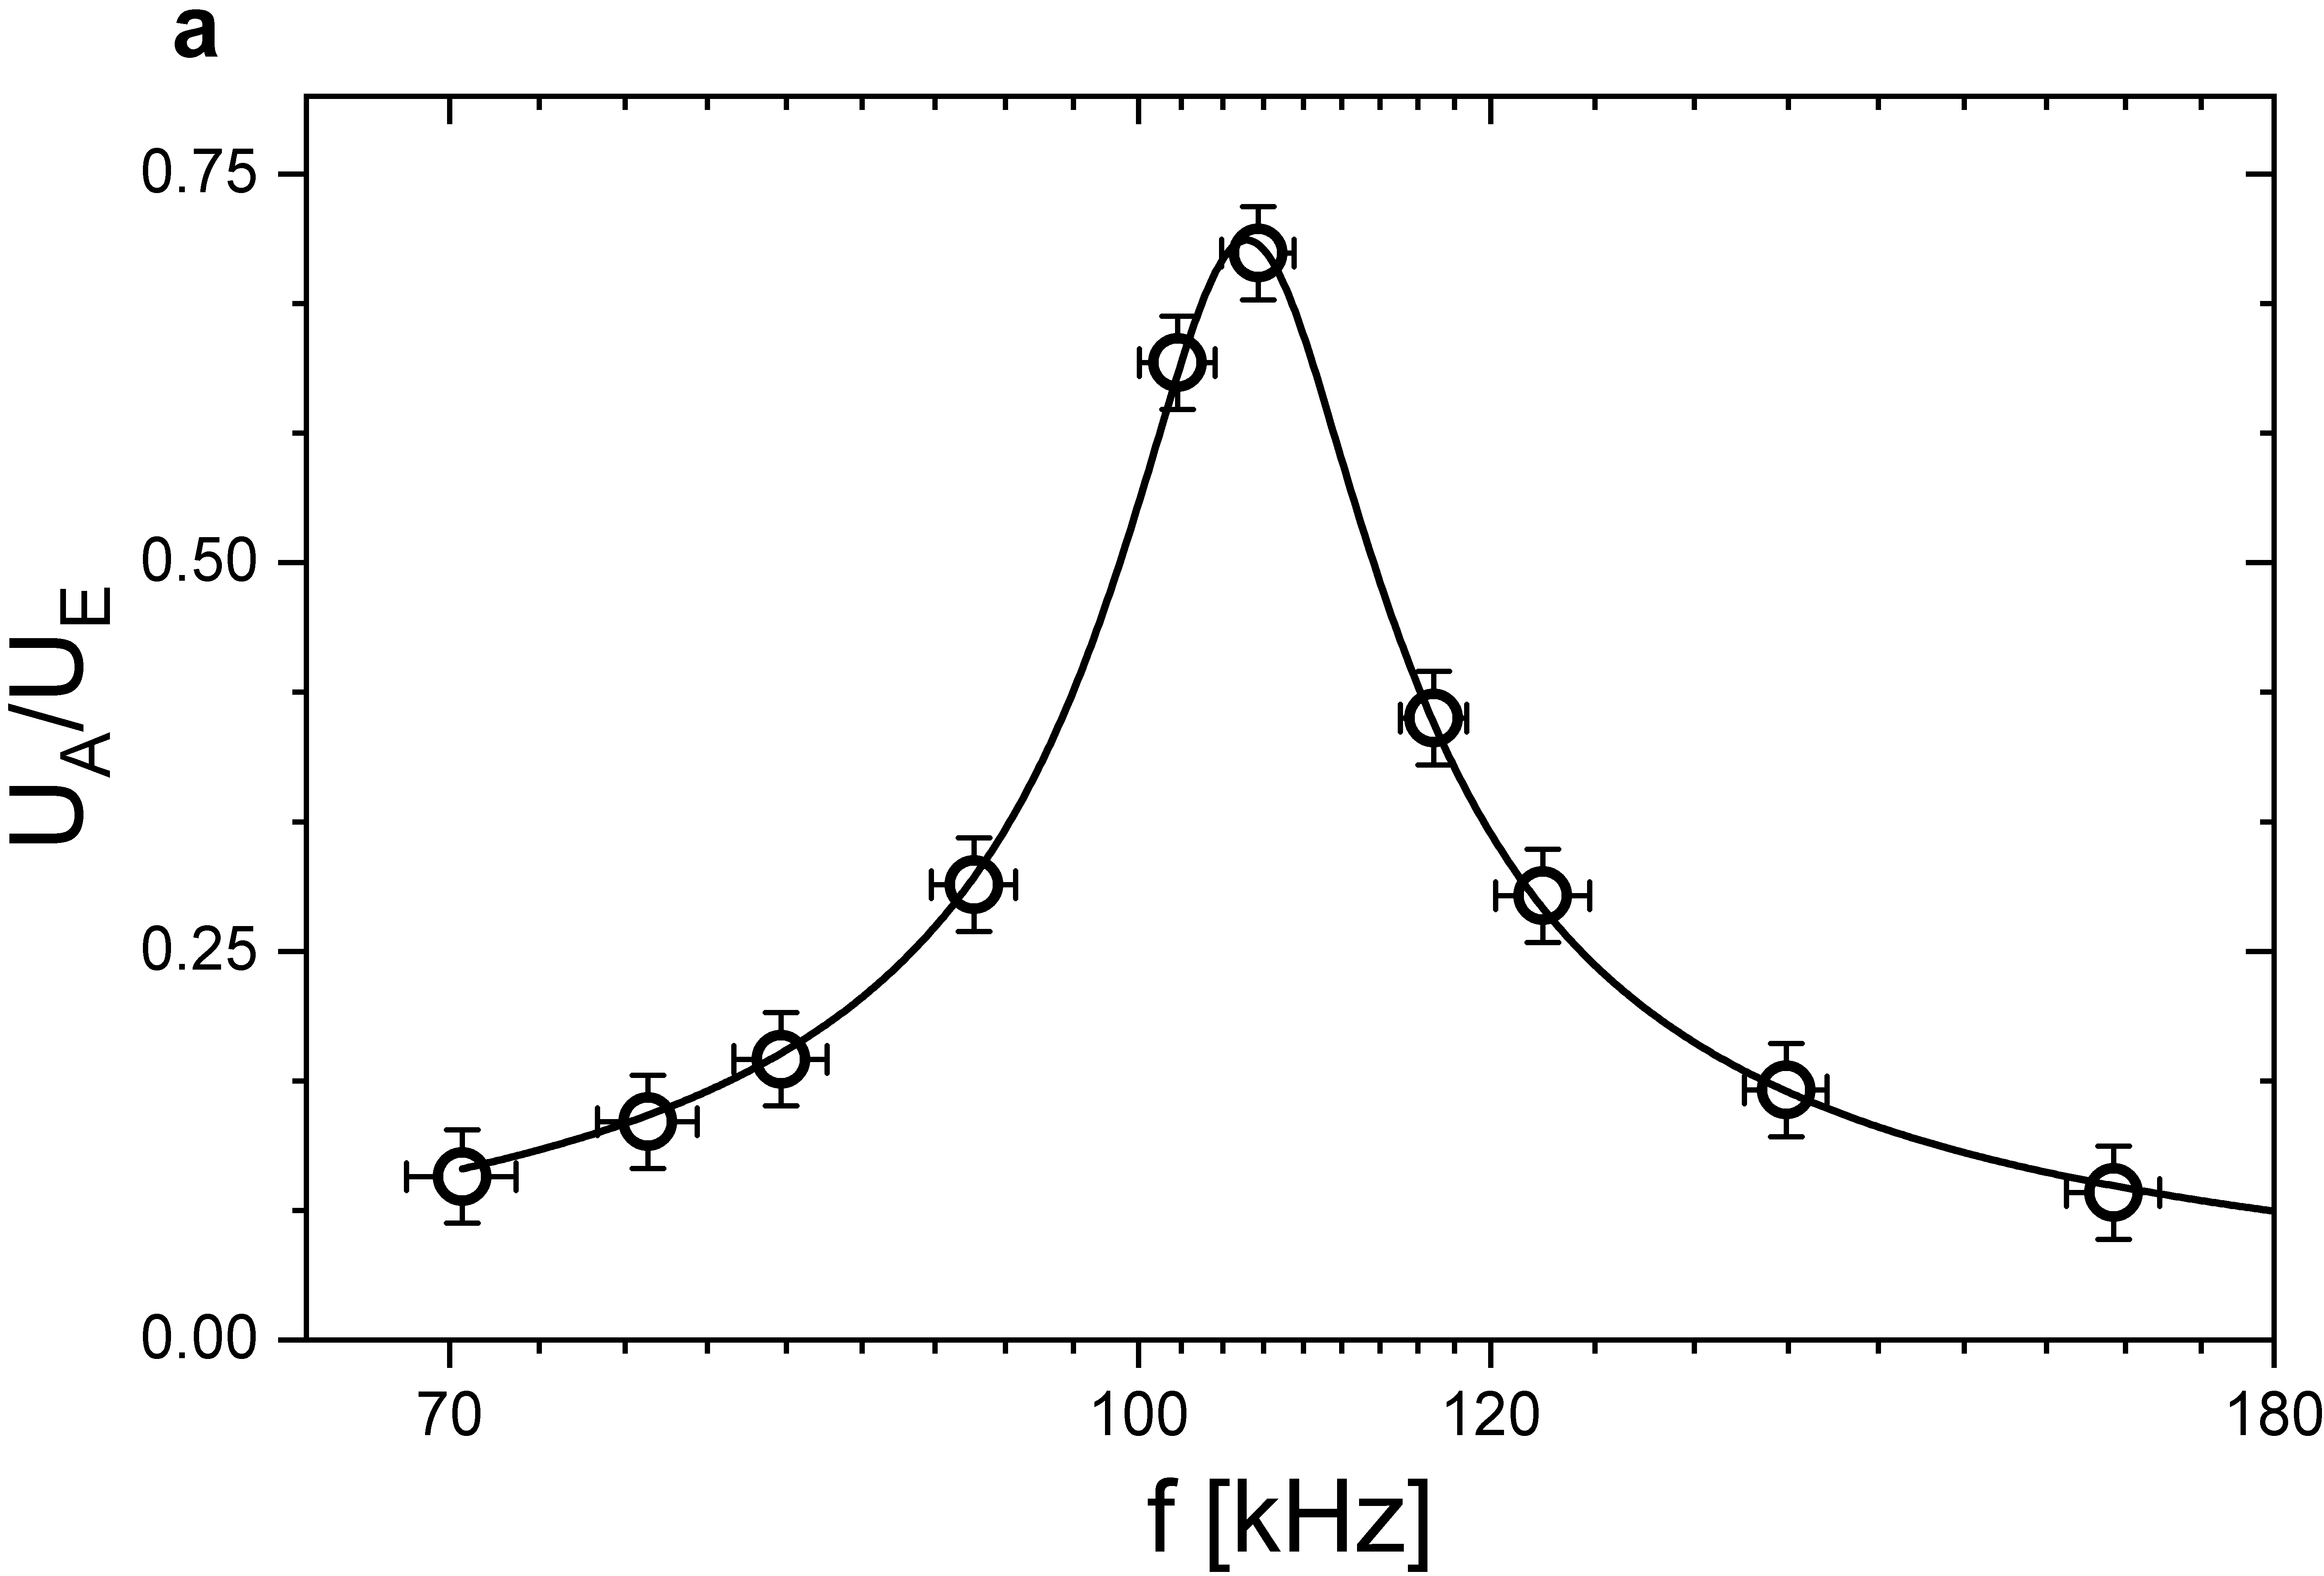
\includegraphics[width=80mm]{graphs/SerieDurch1.png}
                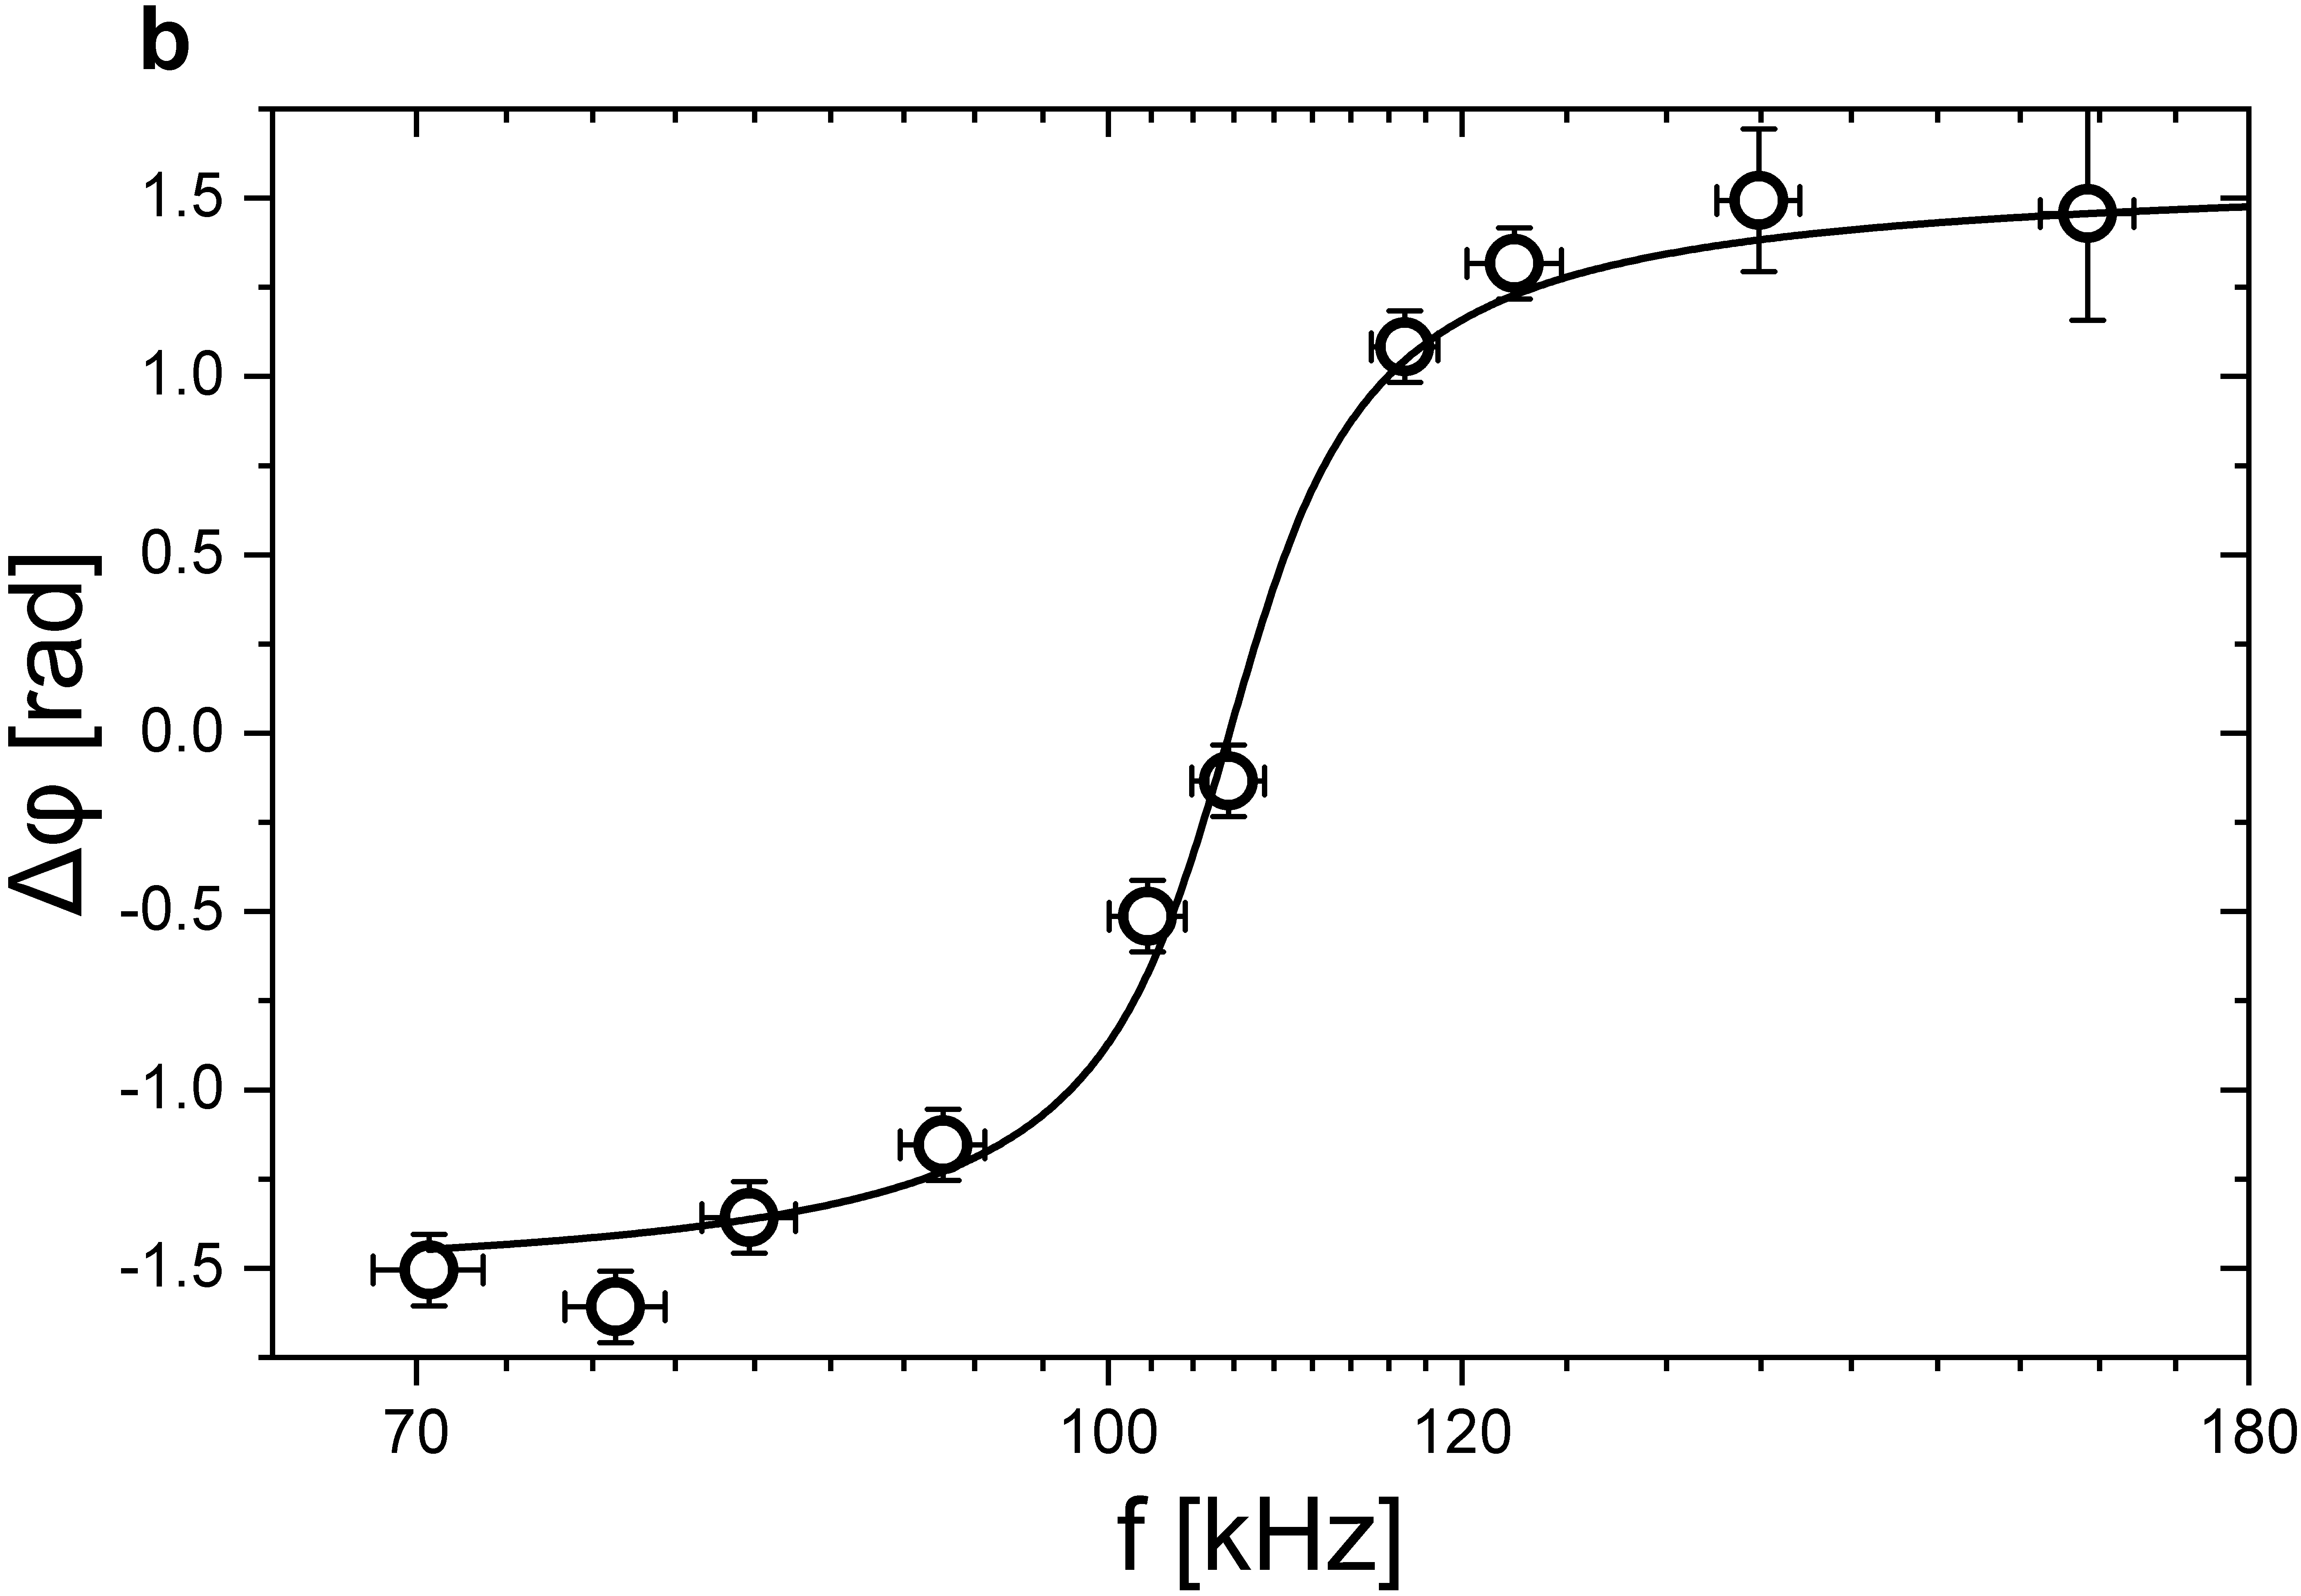
\includegraphics[width=79mm]{graphs/SeriePhase1.png}
                \caption{
                    \textbf{a} Durchlasskurve eines Serienschwingkreis. Die berechnete Resonanzfrequenz liegt hierbei bei $f_g \approx 105$ kHz.
                    \textbf{b} Phasenverschiebung bezügliche Eingangs-/ und Ausgangssignal bei einem Serienschwingkreis. Die berechnete Resonanzfrequenz liegt hierbei bei $f_g \approx 106 $ kHz.\\
                    Bei beiden dargestellten Kurven handelt es sich um die Theoriefunktionen \ref{eq:durchlasskurveSerie}-\ref{eq:phasenkurveSerie}.
                }
                \label{fig:serieKurve}
            \end{figure*}
            
            \begin{table}
                \centering
                \begin{tabular}{c|ccc}
                    \multicolumn{1}{c}{} & \multicolumn{1}{c}{$f_{\mathrm{res}}$ [kHz]} & \multicolumn{1}{c}{$B_f$ [kHz]} & \multicolumn{1}{c}{$Q$} \\
                    \cmidrule(lr){2-2}\cmidrule(lr){3-3} \cmidrule(lr){4-4}
                    \toprule
                    \textbf{a}      & $(98,10 \pm 9,47)$  & $(10,15 \pm 0,27)$ & $(9,65 \pm 0,96)$ \\
                    \textbf{b}      & $(105,75 \pm 11,15)$ & $(13,90 \pm 0,19)$ & $(7,60 \pm 0,80)$ \\
                    \textbf{c}      & $(106,42 \pm 4,40)$ & $(11,21 \pm 0,69)$ & $(9,49 \pm 0,39)$ \\
                    \bottomrule
                \end{tabular}
                \caption{Gesuchte Charakteristiken des verwendeten Serienschwingkreises. Bei den dargestellten Werten handelt es sich bei \textbf{a} um die theoretischen Werte, \textbf{b} experimentell bestimmte Werte mittels Durchlasskurve und \textbf{c} experimentell bestimmte Werte mittels Phasenverschiebungskurve.}
                \label{tab:serie}
            \end{table}
        
        
        \subsection{Dämpfungskonstante}\label{subsec:result_damping}
            Bei der in Kapitel \ref{subsec:result_serie} berechneten Güte handelt es sich um eine Beschreibung der auftretenden Verluste. Dieser Verlust ist Folge der Dämpfung des Serienschwingkreis. Dabei lässt sich diese Dämpfung mittels der Dämpfungskonstante $\delta$ bestimmen. Durch experimentell bestimmte Daten kann diese durch die Steigung einer Ausgleichsgerade bestimmt werden. Hierfür betrachte man Abbildung \ref{fig:damping}.
            Dies ergibt eine experimentell bestimmte Dämpfungskonstante von
            \begin{center}
                $\bm{\delta}$ $\mathbf{ = (20,58 \pm 0,19)}$ \textbf{kHz} $\quad$.
            \end{center}
            Eine theoretische Bestimmung von $\delta$ kann mittels Formel \ref{eq:dampingSerie} durchgeführt werden. Hierfür verwendet man die in Kapitel \ref{subsec:result_serie} aufgeführten Eigenschaften der Bauteile.
            Dies gibt
            \begin{center}
                $\bm{\delta}$ $\mathbf{= (31,91 \pm 0,85)}$ \textbf{kHz} $\quad$.
            \end{center}
            
            \begin{figure}
                \centering
                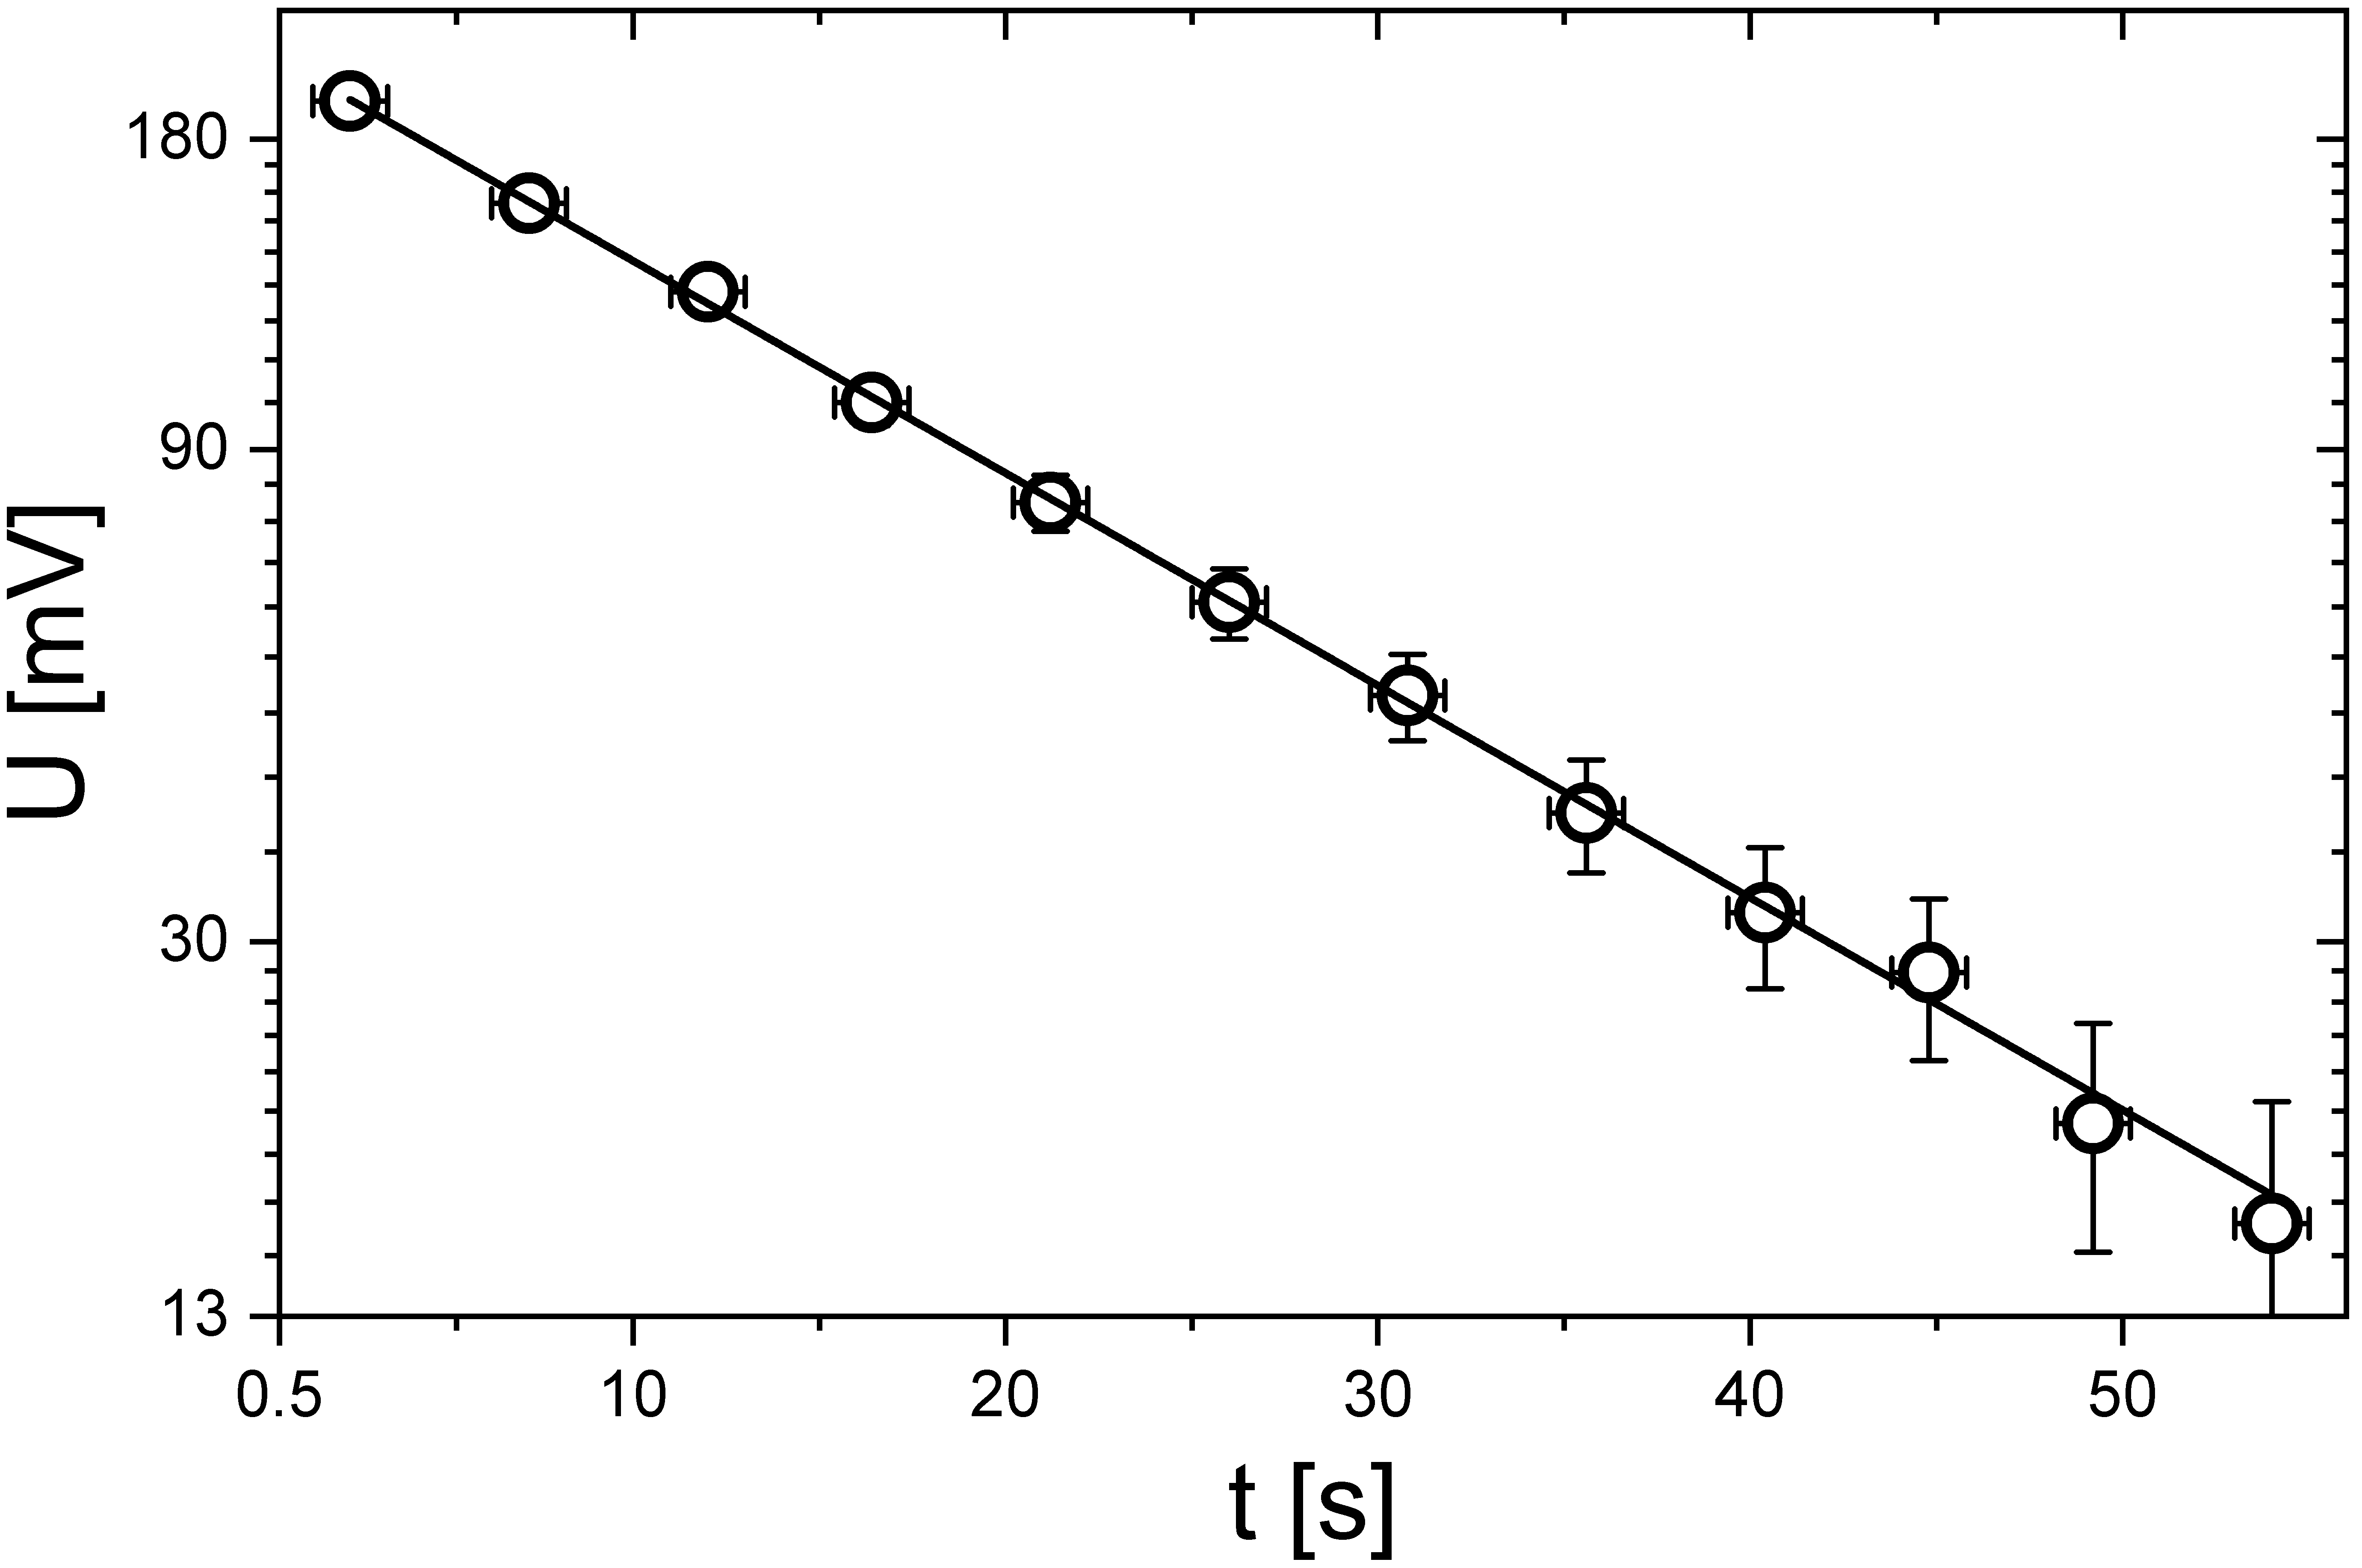
\includegraphics[width=74mm]{graphs/Damping1.png}
                \caption{Halblogarithmische Darstellung der Abnahme der Amplitude gegen deren Zeitabstände. Mittels der Steigung der dargestellten Ausgleichsgerade kann die Dämpfungskonstante bestimmt.}
                \label{fig:damping}
            \end{figure}
            
        
        \subsection{Koaxialkabel}
            Zur Berechnung der Kapazität des Koaxialkabels wird Gleichung \ref{eq:kapschwing} von \ref{eq:kapschwingkoax} abgezogen. Man erhält daraus folgenden Ausdruck. 
            \begin{equation}
                \owncount
                C_{KK} = \frac{1}{L\cdot 4\pi^2}\cdot \left(\frac{1}{f_{res,KK}^2}-\frac{1}{f_{res,S}^2}\right)
                \label{eq:kapkoax}
            \end{equation}\\
            Wie in der Aufgabe beschrieben wurden die Kapazität des Schwingkreises eliminiert. Die Induktivität der Spule war mit $L = (1,000 \pm 0,025)$\,\si{\milli\henry} gegeben. Für die Resonanzfrequenz des Schwingkreises ergaben die Messungen $f_{res,S} = (180,170\pm0,246)$\, \si{\kilo\hertz} und für die Resonanzfrequenz für Schwingkreis mit Koaxialkabel $f_{res,KK} = (119,988 \pm 0,282)$\,\si{\kilo\hertz}. Setzt man diese Werte nun in die oben genannte Formel ergibt sich für die Kapazität 
            \begin{center}
                $\mathbf{C_{KK} = (979,076 \pm 34,878)}$\,\textbf{\si[detect-weight]{\pico\farad}}.
            \end{center}
            Damit kann man den Kapazitätsbelag berechnen. Für ein \SI{10}{\metre} langes Kabel ergibt das folgenden Wert. 
            \begin{equation}
                \owncount
                \frac{C_{KK}}{l} = \frac{979,076\,\si{\pico\farad}}{10\si{\metre}} = 97,9 \si[per-mode = fraction]{\pico\farad\per\metre}
            \end{equation}
    
       
        
    \section{Diskussion}\label{sec:discussion}
    
        \subsection{Tiefpass}\label{subsec:discuss_tiefpass}
            Bei $f_g$ war theoretisch zu erwarten, dass für die Durchlasskurve $U_A = U_E / \sqrt{2}$ gilt, sowie $\varphi = -\frac{\pi}{4} \approx 0,78$. Beide genannten Werte sind in Abbildung \ref{fig:kurve} eingezeichnet. Dabei kommen die experimentell bestimmten Werte sehr nahe an die theoretisch zu erwarteten. Dies bestätigt die Korrektheit der berechneten Ergebnisse.
            \\
            Durch Fitting der Theoriefunktion in die Durchlasskurve, konnte die Grenzfrequenz sehr genau bestimmt werden. Dies bestätigt ein nahezu selbes Ergebnis wie die theoretisch berechnete Grenzfrequenz. Da das Ablesen der Phasenverschiebung mit einer größeren Unsicherheit behaftet ist, konnte $f_g$ in der Phasenverschiebungskurve nur ungenau bestimmt werden. Trotz dessen, kann diese als ungefährer Richtwert dienen.
            
        
        \subsection{Differenzierende und integrierende Wirkung}
            \subsubsection{Tiefpass}
                Wird am Tiefpass ein Signal angelegt, dessen Frequenz weit oberhalb seiner Grenzfrequenz ist, fällt die ganze Eingangsspannung am Widerstand ab während die Ausgangsspannung am Kondensator abgegriffen wird. Daher kann die Eingangsspannung mit der folgenden Formel beschrieben werden.
                \begin{equation}
                    \owncount
                    U_E \approx R\cdot I_{RC} = C \cdot \frac{dU_C}{dt} \cdot R
                    \label{eq:uetief}
                \end{equation}\\
                Es kann die Näherung getroffen werden, dass $U_A \approx U_C$ ist, da die Ausgangsspannung am Kondensator abgegriffen wird. Stellt man nun die Gleichung \ref{eq:uetief} um, kommt man für die Ausgangsspannung auf folgende Form.
                \begin{equation}
                    \owncount
                    U_{A,TP} = \frac{1}{RC} \int U_E dt
                    \label{eq:uatief}
                \end{equation}\\
                Der Tiefpass hat also für $f \gg f_G$ eine integrierende Wirkung.\\
                In \ref{fig:tiefrecht} ist gut zu erkennen, dass ein angelegtes Rechtecksignal bei der Eingangsspannung durch Integration der konstanten Anteile einen linearen Term erzeugt.\\
                Integriert man hingegen ein Dreiecksignal, erhält man aneinandergereihte Parabelstücke, die zusammengesetzt eine Welle ergeben. Dies ist gut in der Abbildung \ref{fig:tiefdrei} zu erkennen.
                
            \subsubsection{Hochpass}
                Sollte am Hochpass ein Signal mit sehr viel niedrigerer Frequenz als die Grenzfrequenz angelegt werden, dann fällt fast die gesamte Eingangsspannung am Kondensator ab. Die Ausgangsspannung wird am Widerstand abgegriffen. Es gilt daher folgende Formel für die Ausgangsspannung. 
                \begin{equation}
                    \owncount
                    U_{A,HP} = R\cdot I_{RC}=RC\dcot \frac{dU_C}{dt} \approx RC\cdot \frac{dU_E}{dt}
                    \label{eq:uahoch}
                \end{equation}\\
                Der Hochpass hat also für $f \ll f_G$ eine differenzierende Wirkung.\\
                In der Abbildung \ref{fig:hochdrei} ist zu erkennen, dass man bei einem Dreieckssignal der Eingangspannung über Differentiation Konstanten erhält. Diese spiegeln sich in einem rechteckförmigen Ausgangssignal wieder. In Abbildung \ref{fig:hochrecht} sieht man, dass eine Differentiation vom Rechtecksignal der Eingangsspannung beim Aufbau der Spannung einen zeitlich kurz andauernden Peak der Ausgangsspannung verursacht, der dann gegen Null läuft. Das ist realistisch, da die Ableitung einer Konstanten Null ist. 
                
                \begin{figure*}
                    \subfloat[Dreieckspannung]{
                        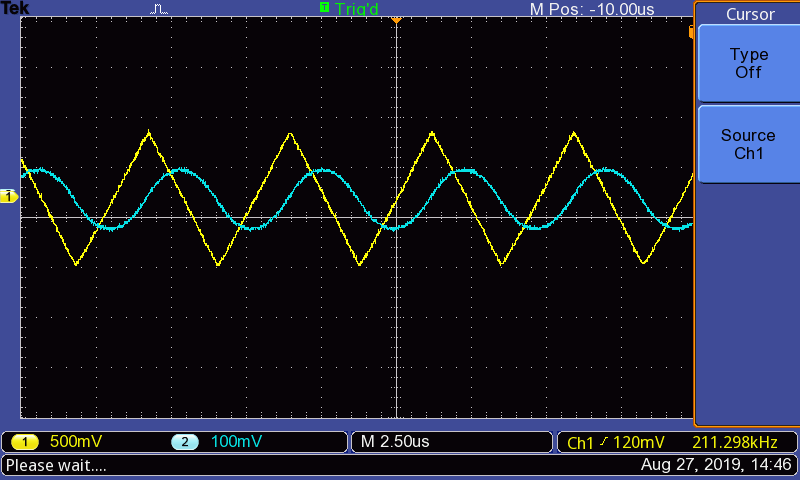
\includegraphics[width=0.45\textwidth]{pictures/Tiefpassdreieck.png}
                        \label{fig:tiefdrei}
                    }
                    \hfill
                    \subfloat[Rechteckspannung]{
                        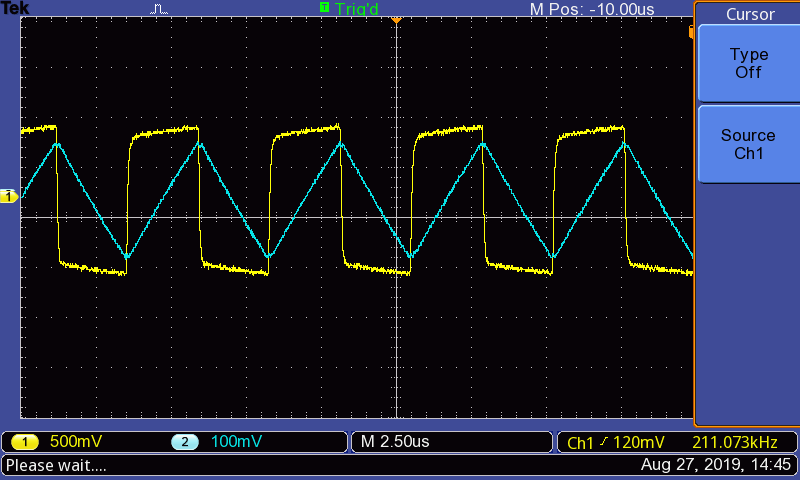
\includegraphics[width=0.45\textwidth]{pictures/Tiefpassrechteck.png}
                        \label{fig:tiefrecht}
                    }
                    \caption{Integrierende Wirkung eines Tiefpasses bei hoher Frequenz. Die Eingangsspannung ist mit gelber Farbe gekennzeichnet, die Ausgangsspannung mit blauer.}
                    \label{fig:tief}
                \end{figure*}
    
            
                \begin{figure*}
                    \subfloat[Dreieckspannung]{%
                        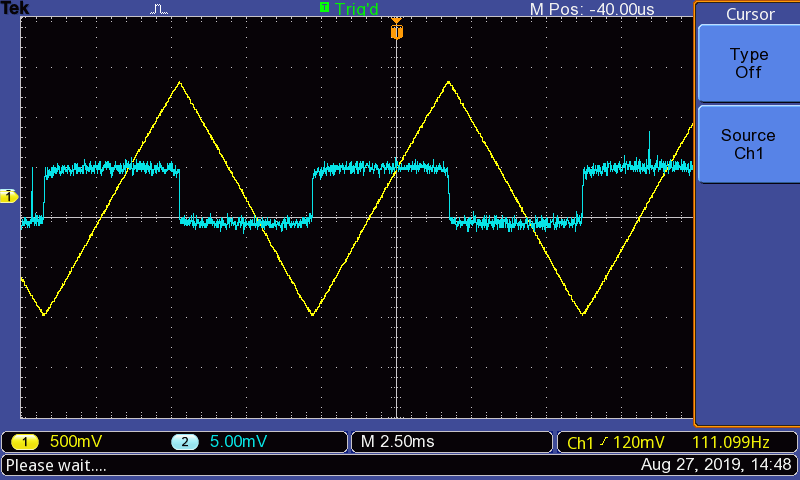
\includegraphics[width=0.45\textwidth]{pictures/Hochpassdreieck.png}
                        \label{fig:hochdrei}
                    }
                    \hfill
                    \subfloat[Rechteckspannung]{%
                        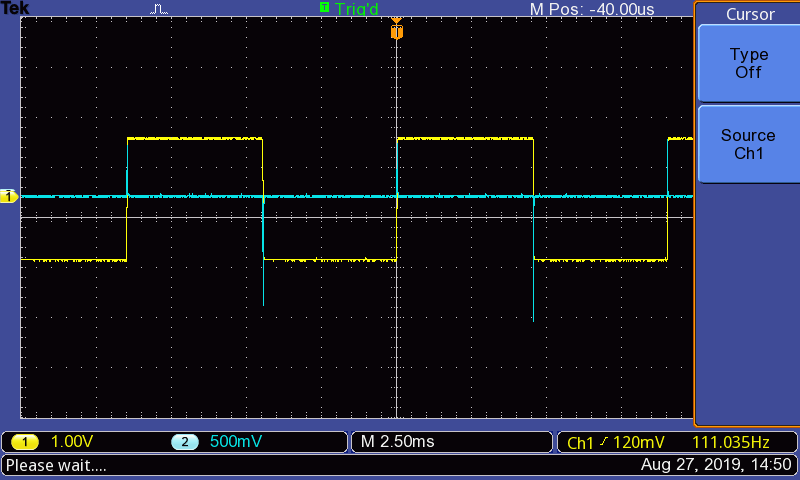
\includegraphics[width=0.45\textwidth]{pictures/Hochpassrechteck.png}
                        \label{fig:hochrecht}
                    }
                    \caption{Differenzierende Wirkung eines Hochpasses bei niedriger Frequenz. Die Eingangsspannung ist mit gelber Farbe gekennzeichnet, die Ausgangsspannung mit blauer.}
                    \label{fig:hoch}
                \end{figure*}
        
    
        \subsection{Serienschwingkreis}
            Bei dem Serienschwingkreis wurden drei verschiedene Charakteristiken mittels drei verschiedenen Methoden bestimmt. Dabei ist die Bestimmung von $f_g$ mittels Durchlasskurve, wie auch in Kapitel \ref{subsec:discuss_tiefpass} bereits angemerkt, genauer, als durch Phasenverschiebungskurve. Die Bandbreite und die Güte konnten anschließend jedoch mittels letzterer Kurve genauer bestimmt werden. Dies liegt daran, dass die gesuchten Parameter der Theoriekurve der Phasenverschiebungskurve genauer bestimmt werden konnten. Hätte man für die Durchlasskurve um $f_g$ mehr Datenpunkte aufgenommen, so wäre eine genauere Bestimmung der verschiedenen Charakteristiken möglich. 
            \\
            In Abbildung \ref{fig:serieKurve} betrachtet man zudem eine scharfe Resonanz, da die Bandbreite etwa 10 \% der Resonanzfrequenz entspricht. Aus dieser scharfen Resonanz folgt somit auch ein relativ hoher Gütefaktor, welcher in Tabelle \ref{tab:serie} dargestellt ist.
            
            
        \subsection{Dämpfungskonstante}
            Die Bestimmung von $\delta$ war sehr gut möglich. Trotzdem ist eine große Diskrepanz zwischen des experimentell und theoretisch berechneten Ergebnis sichtbar. Eine mögliche Ursache für diese große Abweichung ist ein ungenaues Ablesen der Amplituden. Jedoch erlauben vor allem große Amplituden ein gutes Ablesen dieser und deren Zeitabstände. Dies ist in Abbildung \ref{fig:damping} gut sichtbar. Für kleine Amplituden, und somit größeren Zeitabständen, befinden sich die Datenpunkte nicht mehr genau auf der Ausgleichsgerade. Trotz dessen, ist es möglich eine relativ genaue Gerade zu erstellen. Ablesegenauigkeit kann somit als Ursache ausgeschlossen werden.
            \\
            Man bemerke, dass die Dämpfungskonstante bereits in Abbildung \ref{fig:serieKurve}b geschätzt werden kann. Je steiler die Phasenverschiebungskurve im Transferbereich von negativer zu positiver Phasenverschiebung ist, desto kleiner ist $\delta$. Da in diesem Fall die Kurve nicht sehr steil ist, kann von einer relativ schwachen Dämpfung ausgegangen werden. Diese Schätzung bestätigt die berechnete Dämpfungskonstante. Diese bewirkt unter anderem auch das auftreten des Schwingfall. Dieser tritt auf, da $\delta < \frac{1}{LC}$.
            \\
            Ein weitere Kontrolle der Dämpfungskonstante liefert die Benutzung der Bandbreite.
            \begin{equation}
                \owncount
                \delta = B_f \pi
            \end{equation}
            Setzt man hier die in Kapitel \ref{subsec:result_serie} berechneten Werte ein, so ergibt sich in etwa die theoretisch berechnete Dämpfungskonstante. Die Diskrepanz zwischen der Bestimmung mittels Steigung und der Bestimmung mittels Berechnung bleibt weiterhin bestehen.
        
        
        \subsection{Koaxialkabel}
            Die Messergebnisse der Resonanzfrequenzen scheinen realistisch zu sein, wenn man sich die Formel \ref{eq:grenzSerie} ansieht. Es muss bei einer höheren Kapazität eine niedrigere Frequenz folgen. Genau das wurde auch gemessen.\\
            Für die Berechnung der Kapazität des Koaxialkabels wurde der Dämpfungsfaktor vernachlässigt, da es sich hierbei um eine getrieben Schwingung handelt.
            Der Kapazitätsbelag mit \SI[per-mode = fraction]{97,9}{\pico\farad\per\metre} ist für ein Koaxialkabel mit einem Wellenwiderstand von \SI{50}{\ohm} ein realistischer Wert \footnote{\url{https://uol.de/fileadmin/user_upload/physik/ag/physikpraktika/download/GPR/pdf/LC_Ketten_Koaxialkabel.pdf}, Seite 12, zuletzt besucht am 29.08.2019}. Bei einer Gesamtlänge von \SI{10}{\metre} ergibt sich dann eine Kapazität von \SI{979}{\pico\farad}.
            
        
        \subsection{Unterschiede zwischen Schwingkreis, Hoch- und Tiefpass}
            Der Unterschied zwischen Hoch-/Tiefpassen und Schwingkreisen liegt in deren Bauweise. Hoch- und Tiefpasse bestehen aus einem RC-Glied (Widerstand, Kondensator) während ein Schwingkreis aus einem RCL-Glied (Widerstand, Kondensator, Spule) besteht. Aufgrund dieser Bauweise ist es im Schwingkreis möglich die elektrische Energie periodisch in elektrische Feldenergie im Kondensator, sowie in magnetische Feldenergie in der Spule umzuwandeln. Daraus resultiert die Schwingung. Es handelt sich dabei um eine gedämpfte Schwingung, da im ohmschen Widerstand Energie in Wärme umgewandelt wird.\\
            Ein weiterer Unterschied zwischen den drei Bauteilen ist die Durchlässigkeit verschiedener Frequenzen. Der Hochpass lässt nur Frequenzen oberhalb seiner Grenzfrequenz passieren. Alle anderen Signale werden vom Widerstand so stark gedämpft, dass sie am Ausgang fast nicht mehr wahrnehmbar sind. Beim Tiefpass ist es genau umgekehrt. Es werden nur die Frequenzen unterhalb der Grenzfrequenz durchgelassen. Beim Schwingkreis ist der durchgelassene Frequenzbereich abhängig von der Resonanzfrequenz. Entweder werden die Signale in diesem Bereich abgeblockt (Bandsperre) oder durchgelassen (Bandpass).\\
            Der Schwingkreis kommt bei fast allen Sendern und Empfängern zum Einsatz, da einzelne Signale isoliert werden können. Der Hoch- und Tiefpass findet üblicherweise in der Tontechnik Verwendung. 
        
        \subsection{Analogien zwischen Feder-Masse-System und einfachen LRC-Schwingkreisen}
            Die Analogien zwischen den beiden Systemen kann aus Tabelle \ref{tab:anasys} abgelesen werden. \\
            Da beide Systeme schwingfähig sind, können die Differenzialgleichungen verglichen werden. Daran erkennt man die Ähnlichkeit der Systeme. Eine weitere Gemeinsamkeit ist die Transformation der Energie, während einer Periode, in zwei verschiedene Formen.
            \begin{table}
                    \begin{center}
                    \scalebox{1.1}{
                    \begin{tabular}{c|c}
                        \multicolumn{1}{c}{Feder-Masse-System} & \multicolumn{1}{c}{LRC-Schwingkreis}\\
                        \cmidrule(lr){1-1}\cmidrule(lr){2-2}
                        \toprule
                        \textbf{Schwingungsgleichung}  & \textbf{Schwingungsgleichung} \\
                        $m \cdot \ddot{s} + k\cdot \dot{s} + D\cdot s = 0$  & $L\cdot \ddot{Q}+R\cdot\dot{Q}+\frac{1}{C}\cdot Q = 0 $\\
                        Auslenkung s & Ladung Q \\
                        Reibungskoeffizient k & Widerstand R \\
                        Federhärte D & Reziproke Kapazität $\frac{1}{C}$ \\
                        Geschwindigkeit $v (=\dot{s})$ & Stromstärke $I (=\dot{Q})$\\
                        Masse m & Induktivität L \\
                        \hline
                        \textbf{Potenzielle Energie} & \textbf{Energie des elektrischen} \\
                        \textbf{der Felder} & \textbf{Feldes im Kondensator} \\
                        $E_{pot} = \frac{1}{2}\cdot D\cdot s^2$ & $E_{ele} = \frac{1}{2}\cdot C\cdot U^2$\\
                        \hline
                        \textbf{kinetische Energie} & \textbf{Energie des magnetischen} \\
                         & \textbf{Feldes der Spule} \\
                        $E_{kin} = \frac{1}{2}\cdot m\cdot v^2$ & $E_{mag} = \frac{1}{2}\cdot L\cdot I^2$ \\
                        \bottomrule
                    \end{tabular}}
                    \end{center}
                    \caption{Analogien zwischen Feder-Masse-System und einfachen LRC-Schwingkreisen}
                    \label{tab:anasys}
                \end{table}
       
       
       
    \section{Zusammenfassung}\label{sec:conclusion}
        Bei diesem Versuch war die Bestimmung der Eigenschaften von Hoch- und Tiefpass sowie von Schwingkreisen die zentrale Aufgabe. Durch die Bauteile ist es möglich Frequenzen zu filtern bzw. zu isolieren. Sie sind somit von der heutigen Radio- und Tontechnik nicht mehr wegzudenken. 
        % Vielleicht fällt dir noch ein "wichtiges Ergebnis" ein. 
        % Passt schon.



    % References
    \bibliographystyle{mnras}
    \bibliography{Ausarbeitung.bib}
    


    % Appendix
    \appendix
    \section{Fehlerrechnung}\label{subsec:fehler}
        Für die Berechnung der Unsicherheiten wurden die Werte aus \ref{tab:error} als systematische Unsicherheiten verwendet. 
        \begin{table}
            \centering
            \begin{tabular}{c|c}
                \multicolumn{1}{c}{Messgröße} & \multicolumn{1}{c}{Unsicherheit}\\
                \cmidrule(lr){1-1}\cmidrule(lr){2-2}
                \toprule
                Widerstand    & 1\% \\
                Induktivität       & 2,5\%\\
                Kapazität       & 20\% \\
                Frequenz  & \SI{20}{\hertz} \\
                \bottomrule
            \end{tabular}
            \caption{Systematischen Unsicherheiten}
            \label{tab:error}
        \end{table}
        \\
        Die Unsicherheiten der experimentell bestimmten Ergebnisse, sowie der theoretischen Werte, wurde mittels Origin und quadratischer Addition fortgeplanzt. Dabei wurde folgende Formel verwendet.
        \begin{equation}
            \owncount
            \Delta g = \sqrt{\Delta x^2 \left[\frac{\partial g}{\partial x}\right]^2_{x,y,z} + \cdots}
        \end{equation}
        \\
        Beim Tiefpass musste nur die Unsicherheit der Grenzfrequenz berechnet werden.
        \begin{equation}
            \owncount
            \Delta f_g = \sqrt{\Delta R^2 \left|\frac{1}{2\pi R^2C} \right|^2 + \Delta C^2 \left|\frac{1}{2\pi RC^2}\right|^2}
        \end{equation}
        \\
        Für den Serienschwingkreis mussten die Unsicherheiten durch folgende Formeln berechnet werden. Die Berechnung der Unsicherheit der Grenzfrequenz erfolgt analog wie oben.
        \begin{equation}
            \Delta B_f = \sqrt{\Delta R^2 \left|\frac{1}{2\pi L}\right|^2 + \Delta L^2 \left|\frac{R}{2\pi L^2}\right|^2}
        \end{equation}
        \begin{equation}
            \Delta Q = \sqrt{\Delta f_{\mathrm{res}}^2 \left|\frac{1}{B_f}\right|^2 + \Delta B_f^2 \left|\frac{f_{\mathrm{res}}}{B_f^2}\right|^2}
        \end{equation}
        \\
        Die Berechnung der Dämpfung erfolgt analog.
        \begin{equation}
            \Delta \delta = \sqrt{\Delta R^2 \left|\frac{1}{2L}\right|^2 + \Delta L^2 \left|\frac{R}{2L^2}\right|^2}
        \end{equation}

    
    \subsection{Koaxailkabel}
        Zur Ermittlung der statistischen Unsicherheiten der Resonanzfrequenzen wurde die einfache Standardabweichung des Mittelwertes gebildet. Da nur wenige Messergebnisse vorlagen, wurde eine Korrektur mit Hilfe der Student-t-Verteilung, bei vier Messwerten, auf einem Vertrauensniveau von 62,8\% durchgeführt. Für die systematische Unsicherheit der Frequenzen wurde ein Wert von \SI{20}{\hertz} angenommen.\\
        Die Unsicherheit der Kapazität des Kabels wurde unter Verwendung folgender Formel linear fortgepflanzt. 
        \begin{equation}
            \owncount
            \begin{aligned}
                \Delta C_{KK} = \left|\Delta L \frac{1}{L^24\pi^2}\left(\frac{1}{f_{res,KK}}-\frac{1}{f_{res,S}}\right)\right| \\ 
                + \left|\Delta f_{res,S} \frac{1}{L4\pi^2}\frac{-2}{f_{res,S}^3}\right|
                +\left|\Delta f_{res,KK}\frac{1}{L4\pi^2}\frac{-2}{f_{res,KK}}\right|
            \end{aligned}
        \end{equation}
      

    \label{lastpage}
\end{document}
